\documentclass[11pt, a4paper]{article}
\usepackage[utf8]{inputenc}
\usepackage{hyperref}
\usepackage{minted}
\usepackage{graphicx}
\graphicspath{{./images/}}

\begin{document}
\title{Deep Learning}
\author{Samuel Navarro}
\date{\today}
\maketitle

\tableofcontents


\section{Tensorflow}%
\label{sec:tensorflow}


A is a 0-dimensional int32 tensor.

\texttt{A = tf.constant(1234)}

B is a 1-dimensional int32 tensor. 

\texttt{B = tf.constant([123, 456, 789])}

C is a 2-dimensional int32 tensor

\texttt{C = tf.context([ [123, 456, 789], [222, 333, 444] ] ) }


A \textit{Tensorflow Session} as shown above, is an environment for running graph. The session is in charge of allocating the operations to GPUs and/or CPUs, including remote machines. 

What if you want to use a non-constant? 

This is where \texttt{tf.placeholder()} and \texttt{feed\_dict} come into place.

You can't just set \texttt{x} to your dataset and put it in Tensorflow, because over time you'll want your Tensorflow model to take in different datasets with different parameters. You need \texttt{tf.placeholder()}.

\texttt{tf.placeholder()} returns a tensor that gets its value from data passed to the \texttt{tf.session.run()} function, allowing you tu set the input right before the sessions runs. 

\textbf{Session's feed\_dict}

\begin{listing}
\begin{minted}[linenos,numbersep=5pt,frame=lines,framesep=2mm]{python}
x = tf.placeholder(tf.string)
y = tf.placeholder(tf.int32)
z = tf.placeholder(tf.float32)


with tf.Session() as sess:
	output = sess.run(x, feed_dict={x: 'Hello World',
	y: 123, z: 45.67})
\end{minted}
\caption{Feed Dict}
\label{lst:feed_dict}
\end{listing}



\textbf{Tensorflow Linear Function} 

The way you turn your scores into probabilities is using the \textbf{softmax} function. Scores in the context of logistic regression are also called logits.

\textbf{Softmax function}
The softmax function should take in \texttt{x}, a one or two dimensional array of logits. 
In the one dimensional case, the array is just a single set of logits. In the two dimensional case, \textit{each column in the array is a set of logits.} Thats why we use \texttt{axis=0}



What happens to the softmax probabilities when you multiply the logits by 10?

Probabilities get close to 0.0 or 1.0


What happens to the softmax probabilities when you divide the logits by 10?
The probabilities get close to the uniform distribution.

Since all the scores decrease in magnitude, the resulting softmax probabilities will be closer to each other. 

\subsection{Gradient Descent}%
\label{sub:gradient_descent}

One simple principle is that we always want our variables to have zero mean and equal variance whenever possible. This is also good when we do optimization. 

In the case of images, you can do:

$$ \frac{Channel - 128}{128} $$.

And, we also want to have a good weight initialization. There is a lot of methods to make this but for now we can just use the weights from a Gaussian distribution with mean zero and sd sigma.  The sigma values represent the order of magnitude of your output at the initial point of your optimization.

Because of the use of softmax in top of it, the order of magnitude also determines the peakiness of you initial probability distribution. Large sigma means your distribution will have large peaks, very opinitionated. 

A small sigma means that your distributions is very uncertain about things. It's better to begin with uncertain distribution and let the optimization more confident as the training progress. 

So, we should use the small sigma to begin with. 

We need to measure the error on the test data. 

One rule of thumb is that if computing your loss takes n floating points of calculation, computing the gradients takes 3 times that compute. 

And because the loss is huge because it depends on all the data, the gradients could be a very expensive operation. 

In order to same computation power, we can cheat, we can use the average loss for a very small fraction of the training data. (something like from 1 to 1000 training samples). 

The way we pick our samples must be random, in other case it would not work. 

So, the process is like this: \textbf{Stochastic Gradient Descent} 
\begin{enumerate}
	\item Pick a random set of examples. 
	\item Compute the loss for that sample.
	\item Compute the derivative of that sample.
	\item Pretend that that derivate is the right direction to use. (Is not right at all the right direction)
\end{enumerate}

Each calculation is faster because is trained on less data but the price we pay is that we need to take many more steps. 

\textbf{SGD} scales well with model data and model size. But because is fundamentally a pretty bad optimizer, it comes with a lot of issues in practice. 


Tricks to help \textbf{SGD} 
\begin{itemize}
\item Inputs of zero mean and equal variance (small).
\item Initial weigths should be random with mean = 0 and equal variance (small)
\item Momentum: We can run an average of the gradient $M <- 0.9M + \delta L$  Beause the gradient give us the direction, this result in more faster convergence. 
\item Learning Rate Decay: Is benefical to take smaller and smaller steps as you train. Some like to apply an exponential decay to the learning rate, some try to make it smaller every time the learning rate reaches its plateau. There's a lot of ways to go about it but the key thing is to lower every time.
\end{itemize}

About the learning rate tunning, you should never trust how fast you train, it's better to thing on terms of how good you train. 

So, it should be the case that a lower learning rate give us lower loss but in more steps. 


This is why \textbf{SGD} is often refered as black magic. Because you often have many hyperparameters:

\begin{itemize}
	\item initial learning rate
	\item momentum
	\item batch size
	\item weight initialization
\end{itemize}


One of the rules of thumb is that when things don't work, always try to lower your learning rate first. 

\textbf{Adagrad} is a modification of \textbf{SGD} which implicitly does momentum and learning decay for you. 

\subsection{Mini-batching}%
\label{sub:mini_batching}

Is a technique for training on subsets of the dataset instead of all the data at one time. This provides the ability to train a model, even if a computer lacks the memory to store the entire dataset.


Mini-batching is computationally inefficient, since you can't calculate the loss simultaneously across all samples. However, this is a small price to pay in order to be able to run the model at all.

It's also quite useful combined with \textbf{SGD}. The idea is:

\begin{enumerate}
	\item Randomly shuffle the data at the start of each epoch.
	\item Create the mini-batches.
	\item For each mini-batch, you train the network weights with gradient descent. 
\end{enumerate}

Since these batches are random, you're performing \textbf{SGD} with each batch.

Example of the sizes:

\begin{table}[hbt!]
	\centering
	\caption{Float 32 Size}
	\label{tab:float32_size}
	\begin{tabular}{|c|c|c|c|}
		 \hline
		 train\_features & Shape: (55000, 784) & Type: float32  & 172480000 bytes \\
		 \hline
		 train\_labels   & Shape: (55000, 10)  & Type: float32  & 2200000 bytes \\
		 \hline
		 weights		  & Shape: (784,10)	    & Type: float32  & 31360 bytes \\
		 \hline
		 biases		  & Shape: (10,)		& Type: float32  & 40 bytes  \\
		 \hline
	\end{tabular}
\end{table}

In case where the size of the batches would vary, we can take advantage of TensorFlow's \texttt{tf.placeholder()} function to receive the varying batch sizes. 

\texttt{features = tf.placeholder(tf.float32, [None, n\_input])}

\texttt{labels = tf.placeholder(tf.float32, [None, n\_classes])}


The \textbf{None} dimension is a placeholder for the batch size. At runtime, Tensorflow will accept any batch size greater than 0.

\section{Deep Neural Networks}%
\label{sec:deep_neural_networks}



\subsection{Regularization}%
\label{sub:regularization}


\begin{itemize}
	\item Early Termination: We stop training as soon as we stop improving.
	\item Regularization: Applying artificial constraints on my network that implicitly reduce the number of free parameters.
		\begin{itemize}
			\item L2 Regularization: $ \mathcal{L}' = \mathcal{L} + \beta \frac{1}{2} ||\omega||^2_{2}$
		\end{itemize}
	\item Dropout: 
		\begin{itemize}
			\item Image you have one layer that goes to another layer, the values that goes from the next are often called activations, now, take those activations and randomly for every example you train your network, set $p \epsilon \{0, 1\}$ to zero. By doing this,  your network cannot rely on any activation to be present. 
			\item \textbf{If dropout doesn't work, you should probably be using a bigger network.}
			\item  When you want to evaluate your model, you don't want randomness, you want your model to be deterministic. You want to take the consensus over this redundant models. 
			\item You get the consensus by taking the average of the redundant models. 
			\item $y_e \sim E(y_t)$. To make sure this expectation holds:
				\begin{itemize}
					\item During training: Not only zero-out the activation with p probability, but you also scale the remaining activations by a factor of 2 (In this case 2 because we used p=0.5).
				\item In order to compensate for dropped units, \texttt{tf.nn.dropout()} multiplies all units that are kept by \texttt{1 / keep\_drop}  
				\item During validation or testing, you should keep all of the units to maximize accuracy.
			    \end{itemize}
		\end{itemize}

\end{itemize}



Remember that L2 norm stands for:

\[
	\frac{1}{2} (\omega^2_1 + \omega^2_2 + ... + \cdots + \omega^2_{n})
.\] 

This is easy because we can even take the derivate by hand (That is: $\omega$)


\section{Convolutional Neural Networks}%
\label{sec:convolutional_neural_networks}

If you know the structure of your data, it will help a lot for the learning process.

Let's say that you want to classify letters, you already know that the color space doesn't matter in the letters, so, it would be better to use \texttt{R + G + B / 3} instead of the 3 channels. 


Another useful things is \textbf{Translation Invariance}: the idea is that you explicitly tell your network that objects in images are largely the same wherever they appear on the image. (Different positions, same object).

 Another example of \textbf{Translation Invariance} is that when you train a Neural Network in text, most of the time, it doesn't matter whether the Kitten world appears in the text, so you don't need to learn the text Kitten every time it appears on the sentence. 

 The way you achieve this in Neural Networks is using what is called \textbf{Weight Sharing}: When you know that two inputs can contain the same kind of information, you share the weights and train the weights jointly for those inputs. 

 \textbf{Statistical Invariance}: Things that don't change on average across time and space.
 
 For images, the idea of \textbf{Weight Sharing} will get us to study \textit{Convolutional Neural Networks}, for text and sequences in general, in will lead us to embeddings and \textit{Recurrent Neural Networks}


 \textbf{ConvNets:} are Neural Networks that share their parameters across space.\footnote{There's a really clear explanation in the video from the resources}


 \begin{figure}[htb!]
 	\centering
 	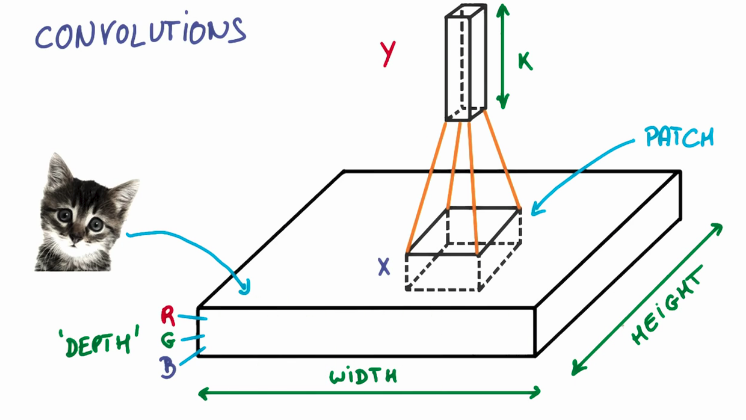
\includegraphics[width=0.8\linewidth]{convolutions}
 	\caption{convolutions}
 	\label{fig:convolutions}
 \end{figure}

 The amount by which the filter slides is referred to as the 'stride'. The stride is a hyperparameter. Increasing the stride reduces the size of your model by reducing the number of total patches each layer observes.

However, this usually comes with a reduction in accuracy.

What's important with the kernels, is that we are grouping together adjacent pixels and treating them as a collective. In a normal, non-convolutional neural network, we would have ignored this adjacency. In a normal network, we would have connected every pixel in the input image to a neuron in the next layer. In doing so, we would not have taken advantage of the fact that pixels in an image are close together for a reason and have special meaning.


\textbf{Filter Depth}

It's common to have more than one filter. Different filters pick up different qualities of a patch. For example, one filter might look for a particular color, while another might look for a kind of object of a specific shape. The amount of filters in a convolutional layer is called the filter depth.


\begin{figure}[htb!]
	\centering
	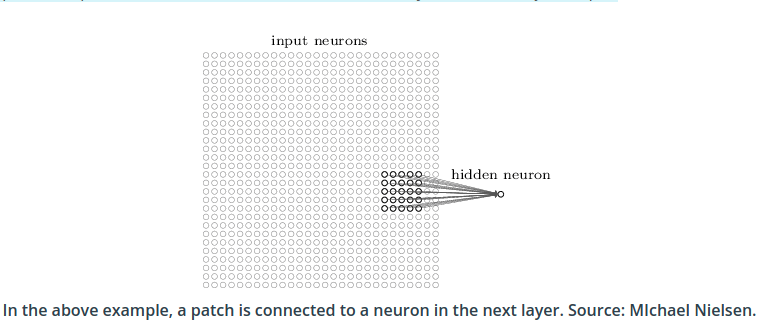
\includegraphics[width=0.8\linewidth]{patch_connection}
	\caption{Patch\_connection}
	\label{fig:patch_connection}
\end{figure}


How many neurons does each patch connect to?

That’s dependent on our filter depth. If we have a depth of \texttt{k}, we connect each patch of pixels to \texttt{k} neurons in the next layer. This gives us the height of \texttt{k} in the next layer, as shown below. In practice, \texttt{k} is a hyperparameter we tune, and most CNNs tend to pick the same starting values.



\begin{figure}[htb!]
	\centering
	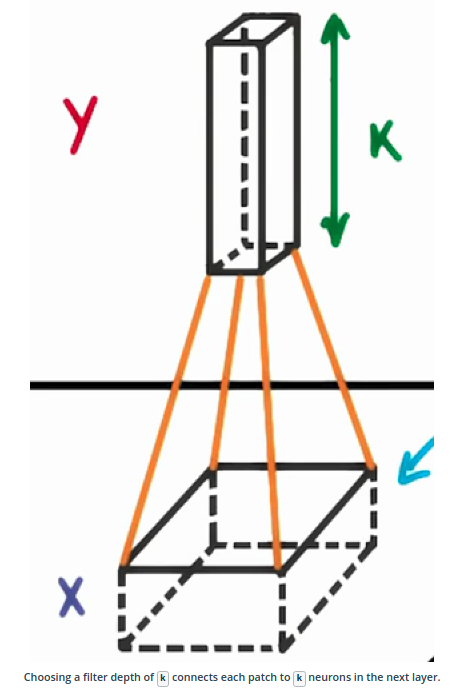
\includegraphics[width=0.8\linewidth]{patch_connection_2}
	\caption{Patch\_Connection}
	\label{fig:patch_connection_2}
\end{figure}


But why connect a single patch to multiple neurons in the next layer? Isn’t one neuron good enough?

Multiple neurons can be useful because a patch can have multiple interesting characteristics that we want to capture.

For example, one patch might include some white teeth, some blonde whiskers, and part of a red tongue. In that case, we might want a filter depth of at least three - one for each of teeth, whiskers, and tongue.

Having multiple neurons for a given patch ensures that our CNN can learn to capture whatever characteristics the CNN learns are important.


\subsection{Parameter Sharing}%
\label{sub:parameter_sharing}

As we saw earlier, the classification of a given patch in an image is determined by the weights and biases corresponding to that patch.

If we want a cat that’s in the top left patch to be classified in the same way as a cat in the bottom right patch, we need the weights and biases corresponding to those patches to be the same, so that they are classified the same way.

This is exactly what we do in CNNs. The weights and biases we learn for a given output layer are shared across all patches in a given input layer. Note that as we increase the depth of our filter, the number of weights and biases we have to learn still increases, as the weights aren't shared across the output channels.

Another thing is that \textbf{sharing parameters} not only helps us with \textbf{translation invariance}, but also give us a smaller, more scalable model.




\subsection{Padding}%
\label{sub:padding}

\begin{figure}[htb!]
	\centering
	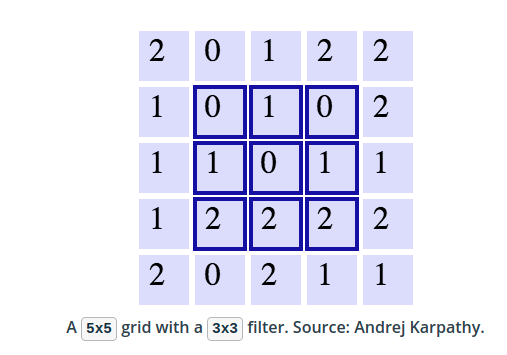
\includegraphics[width=0.8\linewidth]{padding}
	\caption{padding}
	\label{fig:padding}
\end{figure}




We see that we can fit at most three patches in each direction, giving us a dimension of 3x3 in our next layer.


As we can see, the width and height of each subsequent layer decreases in the above scheme. But we want to maintain the same width and height across layers so that we can continue to add layers without worrying about the dimensionality shrinking and so that we have consistency.

One way is to simply add a border of 0s to our original \texttt{5x5} image.\footnote{ \textbf{Valid Padding:} you don't go pass the edge. \textbf{Same Padding:} You go off the edge and put zeros.}


\begin{figure}[htb!]
	\centering
	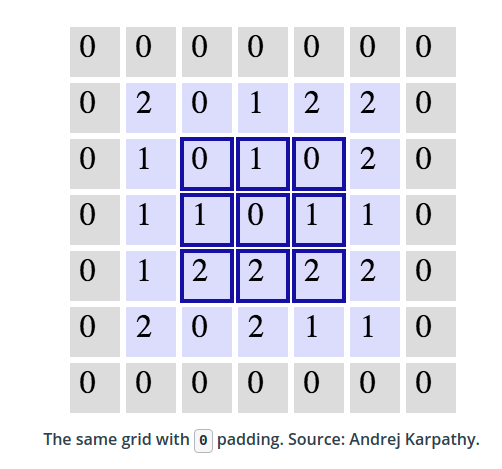
\includegraphics[width=0.8\linewidth]{0_padding}
	\caption{0 Padding}
	\label{fig:0_padding}
\end{figure}



The Figure~\ref{fig:0_padding} ensures that we would expand our original image to a \texttt{7x7}. With this, we now see how our next layer's size is again \texttt{5x5} 


\subsubsection{Dimensionality}%
\label{ssub:dimensionality}

Given:

\begin{itemize}
	\item our input layer has a width of \texttt{W} and a height of \texttt{} 
	\item our convolutional layer has a filter size \texttt{F} 
	\item We have a stride \texttt{S} 
	\item Padding \texttt{P} 
	\item Number of filters \texttt{K} 
\end{itemize}


To obtain the Width or Height of the next layer:

\[
	W/H_{out} =  \frac{W/H-F+2P}{S} + 1
.\] 

The output depth would be equal to the number of filters $D_{out} = K$.

The output volume would be $W_{out} * H_{out} * D_{out}$


Example:


\begin{itemize}
	\item Input shape 32x32x3
	\item 20 filters 8x8x3
	\item Stride 2 for both height and width
	\item Padding = 1
\end{itemize}


The output is 14x14x20, but one important thing to note is that we won't get the same result with Tensorflow because it uses a different algorithm (it uses the \texttt{ceil} of the output)

\begin{listing}
\begin{minted}[linenos,numbersep=5pt,frame=lines,framesep=2mm]{python}
input = tf.placeholder(tf.float32, (None, 32, 32, 3))
# (height, width, input_depth, output_depth)
filter_weights = tf.Variable(tf.truncated_normal((8, 8, 3, 20))) 
filter_bias = tf.Variable(tf.zeros(20))
strides = [1, 2, 2, 1] # (batch, height, width, depth)
padding = 'SAME'
conv = tf.nn.conv2d(input, filter_weights, strides, padding) 
+ filter_bias
\end{minted}
\caption{Convolution Output Shape}
\label{lst:convolution_output_shape}
\end{listing}





Continuing with the example, without parameter sharing, How many parameters does the convolutional layer have?

The \textbf{hint} is that without parameter sharing, each neuron in the output layer must connect to each neuron in the filter. In addition, each neuron in the output layer must also connect to a single bias neuron.


The output layer was of shape: $14x14x20$ so, the answer is:

 \[
	 parameters = (14 * 14 * 20) * (8 * 8 * 3 + 1)  = 756560
.\] 



\textbf{Parameter Sharing}

This is the number of parameters actually used in a convolution layer \texttt{tf.nn.conv2d()}.

Again, the output layer shape is $14x14x20$.

The \textbf{hint} is that with parameter sharing, each neuron in an output channel shares its weights with every other neuron in that channel. So the number of parameters is equal to the number of neuron in the filter, plus a bias neuron, all multiplied by the number fo channels in the output layer. (or, the number of filters?)

\[
 parameters = (8 * 8 * 3 + 1 ) * 20 = 3860 
.\] 

With weight sharing we use the same filter for an entire depth slice. Because of this we can get rid of $14 * 14$ and be left with only 20.




\subsubsection{Tensorflow Convolution Layer}%
\label{ssub:tensorflow_convolution_layer}

The example in Code~\ref{lst:convolution_layer_code} shows Convolutional layers in Tensorflow.

In TensorFlow, \texttt{strides} is an array of 4 elements; the first element in this array indicates the stride for batch and last element indicates stride for features. It's good practice to remove the batches or features you want to skip from the data set rather than use a stride to skip them. 

You can always set the first and last element to \textbf{1} in \texttt{strides} in order to use all batches and features.

The middle two elements are the strides for height and width respectively.


To make life easier, the code is using \texttt{tf.nn.bias\_add()} to add the bias. Using \texttt{tf.add()} doesn't work when the tensors aren't the same shape.


\begin{listing}
\begin{minted}[linenos,numbersep=5pt,frame=lines,framesep=2mm]{python}
# Output depth
k_output = 64

# Image Properties
image_width = 10
image_height = 10
color_channels = 3

# Convolution filter
filter_size_width = 5
filter_size_height = 5

# Input/Image
input = tf.placeholder(
    tf.float32,
    shape=[None, image_height, image_width, color_channels])

# Weight and bias
weight = tf.Variable(tf.truncated_normal(
    [filter_size_height, filter_size_width, color_channels, k_output]))
bias = tf.Variable(tf.zeros(k_output))

# Apply Convolution
conv_layer = tf.nn.conv2d(input, weight, strides=[1, 2, 2, 1], 
padding='SAME')
# Add bias
conv_layer = tf.nn.bias_add(conv_layer, bias)
# Apply activation function
conv_layer = tf.nn.relu(conv_layer)
\end{minted}
\caption{Convolution Layer Code}
\label{lst:convolution_layer_code}
\end{listing}





\subsubsection{Improvements}%
\label{ssub:improvements}

\textbf{Pooling}

By now, the way we reduce the feature map size. But this is a very aggressive way to do it because we lose a lot of information. We can run with a very small stride (of 1) but then took all the convolutions in a neighborhood and combine them.

The most common way to go about \textbf{pooling} is max pooling:

$y = max(X_i)$ 

Characteristics of using max pooling:
\begin{itemize}
	\item Parameter free
	\item Often more accurate
	\item more expensive (¿?) But why? If we just said that it was parameter free.
	\item more Hyper parameters. 
		\begin{itemize}
			\item Pooling Size
			\item Pooling Stride
		\end{itemize}
\end{itemize}



Conceptually, the benefit of the max pooling operation is to reduce the size of the input, and allow the neural network to focus on only the most important elements. \textbf{Max Pooling} does this by only retaining the maximum value for each filtered area, and removing the remaining values.



\begin{figure}[htb!]
	\centering
	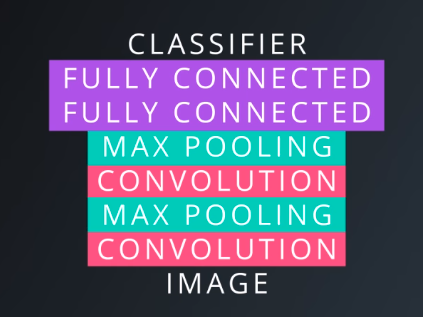
\includegraphics[width=0.8\linewidth]{conv_arch}
	\caption{ConvNet Architecture}
	\label{fig:conv_arch}
\end{figure}



Another form of pooling is average pooling:
$ y = mean(X_i)$

It's a little more like providing a blur low resolution view of the feature map.

The next Code~\ref{lst:max_pooling} we can see an implementation of \texttt{max pooling}. 2x2 filters with a stride of 2x2 are common in practice for max pooling.

The \texttt{ksize} and \texttt{strides} parameters are structured as 4-element lists. \texttt{[batch, height, width, channels]}.

For both \texttt{ksize} and \texttt{strides}, the batch and channel dimensions are typically set to \texttt{1}.

\begin{listing}
\begin{minted}[linenos,numbersep=5pt,frame=lines,framesep=2mm]{python}

conv_layer = tf.nn.conv2d(input, weight, strides=[1, 2, 2, 1], 
padding='SAME')
conv_layer = tf.nn.bias_add(conv_layer, bias)
conv_layer = tf.nn.relu(conv_layer)
# Apply Max Pooling
conv_layer = tf.nn.max_pool(
    conv_layer,
    ksize=[1, 2, 2, 1],
    strides=[1, 2, 2, 1],
    padding='SAME')

\end{minted}
\caption{Max Pooling}
\label{lst:max_pooling}
\end{listing}



\textbf{Pooling Layers} are generally used to: decrease the size of the output and prevent overfitting.

Reducing overfitting is a consequence of the reducing the output size, which in turn, reduces the number of parameters in future layers.


Recently, \textbf{pooling layers} have fallen out of favor. Some reasons are:

\begin{itemize}
	\item Recent datasets are so big and complex we're more concerned about underfitting.
	\item Dropout is a much better regularizer. 
	\item Pooling results in a loss of information. Think about the max pooling operation as an example. We only keep the largest of \textit{n} numbers, thereby disregarding n-1 numbers completely.
\end{itemize}


To calculate the numbers given the max pooling layers, say we have this:

\begin{itemize}
	\item We have an input of shape 4x4x5
	\item Filter of shape 2x2
	\item A stride of 2 for both the height and width
\end{itemize}

Note: For a pooling layer, the output depth is the same as the input depth. Additionally, the pooling operation is applied individually for each depth slice. 

The shape of the output is. 2x2x5.


\textbf{1x1 Convolutions}

The classic convolution it's basically a small classifier for a patch of the image but it's only a \textbf{linear classifier} But if you add a 1x1 convolution in the middle, you now have a mini neural network running over the patch instead of a linear classifier. 


\begin{figure}[htb!]
	\centering
	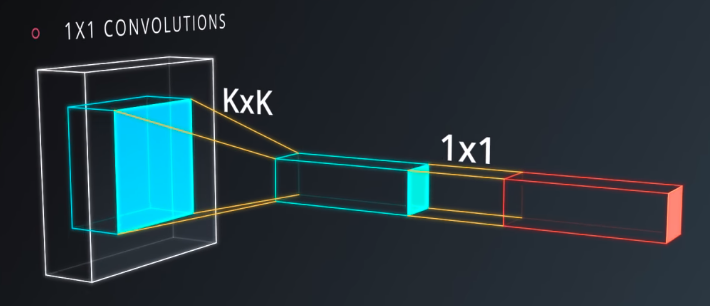
\includegraphics[width=0.8\linewidth]{1x1_conv}
	\caption{1x1 Convolution}
	\label{fig:1x1conv}
\end{figure}


Interspersing your convolutions with 1x1 convolutions is a very inexpensive way to make your models deeper and have more parameters without completely changing the structure. They're also very cheap (they are not convolutions, they are just matrix multiplies and they have relatively few parameters.) 


\textbf{Inception Module}

 The idea is that, at each layer of your ConvNet, usually you need to pick between different options: pooling, 1x1 convolution, 5x5 convolution, etc.

 Instead of that, let's just make a composition of all these choices. This is represented in Figure~\ref{fig:inception}.


 \begin{figure}[htpb!]
 	\centering
 	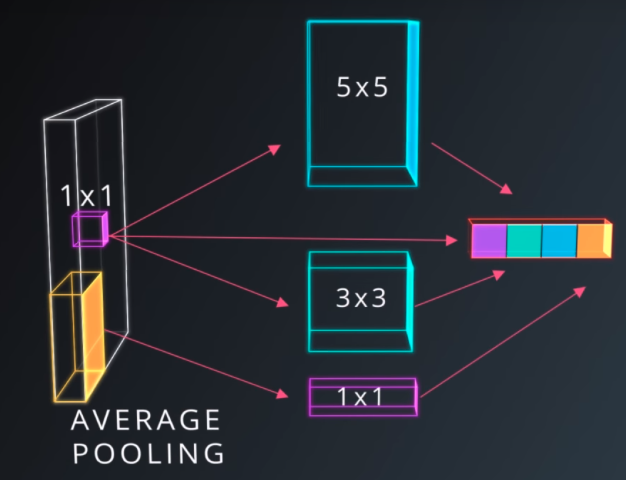
\includegraphics[width=0.8\linewidth]{inception}
 	\caption{Inception}
 	\label{fig:inception}
 \end{figure}


At the top, you simply concatenate the output of each operator. 

You can choose this parameters in such a way that the total number of parameters in your model is very small, yet the model performs better than if you had a simple convolution. 



















\end{document}
